\documentclass[12pt, a4paper]{article}
% Shared preamble — included by all Durin's Code LaTeX documents
\usepackage[a4paper, margin=2.5cm]{geometry}
\usepackage{amsmath, amssymb}
\usepackage{graphicx}
\usepackage{xcolor}
\usepackage{listings}
\usepackage{booktabs}
\usepackage{longtable}
\usepackage{array}
\usepackage{enumitem}
\usepackage{titlesec}
\usepackage{fancyhdr}
\usepackage{hyperref}
\usepackage{fontenc}
\usepackage{inputenc}
\usepackage{microtype}
\usepackage{caption}
\usepackage{subcaption}
\usepackage{tikz}
\usepackage{forest}
\usepackage{mdframed}
\usetikzlibrary{arrows.meta, positioning, shapes.geometric, fit, backgrounds}

% ── Colour palette ──────────────────────────────────────────────
\definecolor{durins-blue}{RGB}{31, 78, 121}
\definecolor{durins-gold}{RGB}{180, 130, 20}
\definecolor{durins-gray}{RGB}{90, 90, 90}
\definecolor{code-bg}{RGB}{248, 248, 248}
\definecolor{code-kw}{RGB}{0, 0, 180}
\definecolor{code-str}{RGB}{163, 21, 21}
\definecolor{code-cmt}{RGB}{0, 128, 0}
\definecolor{code-num}{RGB}{9, 134, 88}

% ── Listings style ──────────────────────────────────────────────
\lstdefinelanguage{DurinsCode}{
  morekeywords={room, action, item, npc, exit, if, else, print, remove,
                player, true, false, description, current_room},
  morestring=[b]",
  morecomment=[l]{//},
  sensitive=true
}
\lstdefinestyle{dc}{
  language=DurinsCode,
  backgroundcolor=\color{code-bg},
  basicstyle=\ttfamily\small,
  keywordstyle=\color{code-kw}\bfseries,
  stringstyle=\color{code-str},
  commentstyle=\color{code-cmt}\itshape,
  numberstyle=\tiny\color{durins-gray},
  numbers=left,
  numbersep=8pt,
  breaklines=true,
  frame=single,
  framerule=0.5pt,
  rulecolor=\color{durins-blue!40},
  xleftmargin=1.5em,
  aboveskip=0.8em,
  belowskip=0.8em,
  tabsize=4,
  showstringspaces=false,
  captionpos=b,
}
\lstdefinestyle{cpp}{
  language=C++,
  backgroundcolor=\color{code-bg},
  basicstyle=\ttfamily\footnotesize,
  keywordstyle=\color{code-kw}\bfseries,
  stringstyle=\color{code-str},
  commentstyle=\color{code-cmt}\itshape,
  numberstyle=\tiny\color{durins-gray},
  numbers=left, numbersep=8pt,
  breaklines=true,
  frame=single, framerule=0.5pt,
  rulecolor=\color{durins-blue!40},
  xleftmargin=1.5em,
  aboveskip=0.8em, belowskip=0.8em,
  tabsize=4, showstringspaces=false,
  captionpos=b,
}
\lstdefinestyle{bash}{
  language=bash,
  backgroundcolor=\color{code-bg},
  basicstyle=\ttfamily\small,
  keywordstyle=\color{code-kw},
  breaklines=true,
  frame=single, framerule=0.5pt,
  rulecolor=\color{durins-blue!40},
  xleftmargin=1.5em,
  numbers=none,
  aboveskip=0.8em, belowskip=0.8em,
  showstringspaces=false,
  captionpos=b,
}

% ── Section formatting ──────────────────────────────────────────
\titleformat{\section}
  {\color{durins-blue}\Large\bfseries}{{\thesection}}{1em}{}[\color{durins-blue}\titlerule]
\titleformat{\subsection}
  {\color{durins-blue!80}\large\bfseries}{{\thesubsection}}{1em}{}
\titleformat{\subsubsection}
  {\color{durins-gray}\normalsize\bfseries}{{\thesubsubsection}}{1em}{}

% ── Header / footer ─────────────────────────────────────────────
\pagestyle{fancy}
\fancyhf{}
\fancyhead[L]{\small\color{durins-gray}Durin's Code — CS4031 Compiler Construction}
\fancyhead[R]{\small\color{durins-gray}\leftmark}
\fancyfoot[C]{\small\color{durins-gray}\thepage}
\renewcommand{\headrulewidth}{0.4pt}
\renewcommand{\footrulewidth}{0.4pt}

% ── Hyperlink style ─────────────────────────────────────────────
\hypersetup{
  colorlinks=true,
  linkcolor=durins-blue,
  urlcolor=durins-blue,
  citecolor=durins-gold,
  pdftitle={Durin's Code — CS4031},
  pdfauthor={Huzaifa Abdul Rehman, Abdul Moiz Hussain, Muhammad Abdullah Khan},
}

% ── Handy boxes ────────────────────────────────────────────────
\newmdenv[
  linecolor=durins-blue!60,
  backgroundcolor=durins-blue!5,
  roundcorner=4pt,
  leftmargin=0, rightmargin=0,
  innerleftmargin=10pt, innerrightmargin=10pt,
  innertopmargin=8pt, innerbottommargin=8pt,
]{infobox}


\begin{document}

% ════════════════════════════════════════════════════════════════
%  TITLE PAGE
% ════════════════════════════════════════════════════════════════
\begin{titlepage}
  \centering
  \vspace*{2cm}
  {\color{durins-blue}\rule{\linewidth}{2pt}}\\[1em]
  {\Huge\bfseries\color{durins-blue} Durin's Code}\\[0.5em]
  {\LARGE\color{durins-gold} Compiler Architecture Document}\\[1em]
  {\color{durins-blue}\rule{\linewidth}{2pt}}\\[2em]

  {\large CS4031 --- Compiler Construction \\ Spring 2026}\\[3em]

  \begin{tabular}{ll}
    \toprule
    \textbf{Student Name} & \textbf{Student ID} \\
    \midrule
    Huzaifa Abdul Rehman   & 23K-0782 \\
    Abdul Moiz Hussain     & 23K-0553 \\
    Muhammad Abdullah Khan & 23K-0607 \\
    \bottomrule
  \end{tabular}

  \vfill
  {\small\color{durins-gray} Document version 1.0 \quad|\quad \today}
\end{titlepage}

\tableofcontents
\newpage

% ════════════════════════════════════════════════════════════════
\section{Overview}
% ════════════════════════════════════════════════════════════════

The Durin's Code compiler is organised as a linear seven-phase pipeline.
Each phase has a well-defined input type and output type; phases communicate only
through these typed interfaces, enabling independent development and testing.

\begin{figure}[h]
\centering
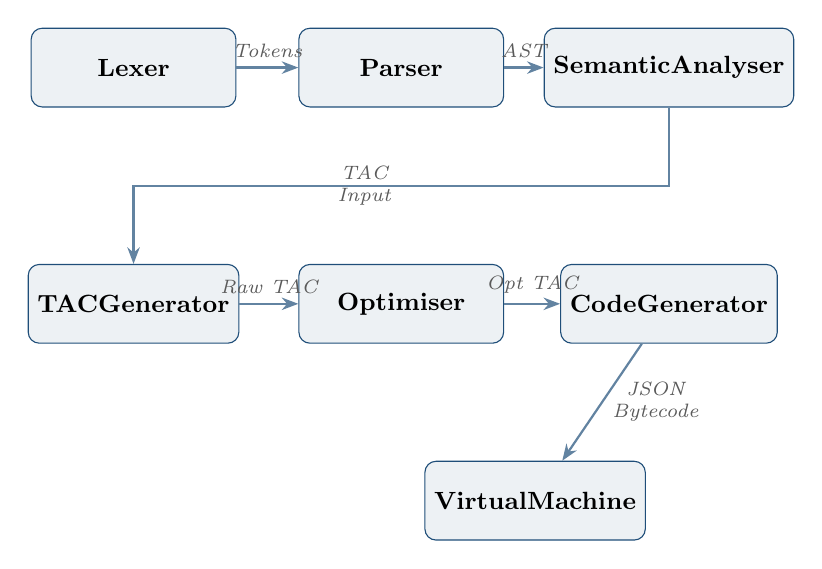
\begin{tikzpicture}[
  box/.style={rectangle, draw=durins-blue, fill=durins-blue!8,
              rounded corners=4pt, minimum width=2.6cm, minimum height=1cm,
              text centered, font=\small\bfseries},
  arr/.style={-{Stealth[length=6pt]}, thick, color=durins-blue!70},
  lbl/.style={font=\scriptsize\itshape, color=durins-gray, align=center}
]
  \node[box] (lex)  at (0,0)    {Lexer};
  \node[box] (par)  at (3.4,0)  {Parser};
  \node[box] (sem)  at (6.8,0)  {Semantic\\Analyser};
  \node[box] (tac)  at (0,-3)   {TAC\\Generator};
  \node[box] (opt)  at (3.4,-3) {Optimiser};
  \node[box] (cg)   at (6.8,-3) {Code\\Generator};
  \node[box] (vm)   at (5.1,-5.5) {Virtual\\Machine};

  \draw[arr] (lex) -- node[above,lbl]{Tokens} (par);
  \draw[arr] (par) -- node[above,lbl]{AST} (sem);
  \draw[arr] (sem) -- ++(0,-1.5) -| node[near start, left, lbl]{TAC\\Input} (tac);
  \draw[arr] (tac) -- node[above,lbl]{Raw TAC} (opt);
  \draw[arr] (opt) -- node[above,lbl]{Opt TAC} (cg);
  \draw[arr] (cg)  -- node[right,lbl]{JSON\\Bytecode} (vm);
\end{tikzpicture}
\caption{Durin's Code compilation pipeline}
\end{figure}

\begin{center}
\begin{tabular}{clll}
\toprule
\textbf{\#} & \textbf{Phase} & \textbf{Input} & \textbf{Output} \\
\midrule
1 & Lexer             & Raw source \texttt{char*}  & \texttt{Token} stream \\
2 & Parser            & \texttt{Token} stream       & \texttt{ProgramNode} AST \\
3 & Semantic Analyser & \texttt{ProgramNode}         & \texttt{SemanticResult} + \texttt{SymbolTable} \\
4 & TAC Generator     & AST + \texttt{SymbolTable}  & \texttt{TACProgram} \\
5 & Optimiser         & \texttt{TACProgram}          & Optimised \texttt{TACProgram} \\
6 & Code Generator    & AST + \texttt{TACProgram}   & JSON bytecode string \\
7 & Virtual Machine   & JSON bytecode                & Interactive game session \\
\bottomrule
\end{tabular}
\end{center}

% ════════════════════════════════════════════════════════════════
\section{Phase 1 --- Lexer}
% ════════════════════════════════════════════════════════════════

\subsection{Responsibility}
Convert a null-terminated C-string source into \texttt{Token} structs on demand
(\emph{pull model} --- \texttt{scanToken()} is called once per token, lazily).

\subsection{Data Structures}

\begin{lstlisting}[style=cpp, caption={Lexer state and Token struct}]
struct Lexer {
    const char* start;      // start of current lexeme
    const char* current;    // scan head
    int line, column;
    TokenType lastEmitted;
    TokenType lastBeforeDot; // for context-sensitive dot handling
};

struct Token {
    TokenType   type;
    const char* start;   // pointer into original source (no copy)
    int         length;
    int         line, column;
};
\end{lstlisting}

\subsection{Key Design Decisions}

\paragraph{Pull model.}
The parser calls \texttt{scanToken()} whenever it needs the next token.
There is no buffering; the lexer reads one character at a time.
This minimises memory use for large source files.

\paragraph{Context-sensitive dot tokens.}
When a \texttt{.} is scanned, \texttt{lastBeforeDot} records the previous token type.
The next identifier is reclassified:
\begin{itemize}
  \item \texttt{player.}\textit{x} $\Rightarrow$ \texttt{TOKEN\_PLAYER\_ATTR}
  \item \textit{id}\texttt{.}\textit{x} $\Rightarrow$ \texttt{TOKEN\_ROOM\_ATTR}
\end{itemize}
This avoids adding semantic lookahead to the parser.

\paragraph{Line/column tracking.}
The \texttt{advance()} function is the single point that increments
\texttt{lexer.line} and resets \texttt{lexer.column} on \texttt{\textbackslash n}.
No other function touches these counters, preventing double-counting bugs.
Windows \texttt{\textbackslash r\textbackslash n} endings are consumed as a single newline.

\paragraph{Error recovery.}
A lexer error emits a \texttt{TOKEN\_ERROR} token pointing to a static error string.
Scanning stops; the parser detects \texttt{TOKEN\_ERROR} and reports the failure.

% ════════════════════════════════════════════════════════════════
\section{Phase 2 --- Parser}
% ════════════════════════════════════════════════════════════════

\subsection{Responsibility}
Consume the token stream and build a fully typed Abstract Syntax Tree
rooted at \texttt{ProgramNode}.

\subsection{Algorithm}
Hand-written recursive descent. Each grammar production maps 1-to-1 to a
\texttt{parseXxx()} function. No parser-generator is used.

\subsection{AST Node Hierarchy}

\begin{lstlisting}[style=cpp, caption={AST node types (simplified)}]
struct ASTNode {
    NodeType type;
    int line, column;
};

struct ProgramNode : ASTNode {
    std::vector<std::unique_ptr<ASTNode>> declarations;
};

struct RoomDeclNode : ASTNode {
    std::string name, description;
    std::vector<std::unique_ptr<ItemDeclNode>> items;
    std::vector<std::unique_ptr<NpcDeclNode>>  npcs;
    std::vector<std::unique_ptr<ExitDeclNode>> exits;
};

struct ActionDeclNode : ASTNode {
    std::string name;
    std::vector<std::unique_ptr<StmtNode>> body;
};

// Statements: PrintStmtNode, RemoveStmtNode, AssignStmtNode, IfStmtNode
// Conditions: ConditionNode { type, lhs, rhs, left, right }
\end{lstlisting}

All child ownership is expressed through \texttt{unique\_ptr}.
There is no manual \texttt{delete} anywhere in the parser.

\subsection{Error Recovery}
On a parse error the parser calls \texttt{synchronize()}, which advances past
statement-boundary tokens (\texttt{\}}, \texttt{room}, \texttt{action}).
This allows multiple parse errors to be reported in a single compilation.

% ════════════════════════════════════════════════════════════════
\section{Phase 3 --- Semantic Analyser}
% ════════════════════════════════════════════════════════════════

\subsection{Responsibility}
Statically validate the AST against all language rules and produce a
\texttt{SymbolTable} consumed by downstream phases.

\subsection{Two-Pass Design}

The analyser runs two passes over the AST:

\begin{center}
\begin{tabular}{clp{8cm}}
\toprule
\textbf{Pass} & \textbf{Function} & \textbf{Action} \\
\midrule
1 & \texttt{registerDeclarations()} &
  Walk all top-level declarations; insert rooms, items, NPCs, and actions into
  the \texttt{SymbolTable}. Report duplicates. \\
\midrule
2 & \texttt{validateDeclarations()} &
  For each room: verify exit targets exist and no direction is repeated.
  For each action: validate \texttt{remove}, \texttt{has\_item}, and
  \texttt{current\_room} references. \\
\bottomrule
\end{tabular}
\end{center}

A two-pass design is necessary because exits may reference rooms declared later
in the file.  A single-pass approach would incorrectly report forward references
as errors.

\subsection{Symbol Table}

\begin{lstlisting}[style=cpp, caption={SymbolTable structure}]
struct SymbolTable {
    std::unordered_map<std::string, RoomInfo>   rooms;
    std::unordered_map<std::string, ItemInfo>   items;
    std::unordered_map<std::string, NpcInfo>    npcs;
    std::unordered_map<std::string, ActionInfo> actions;
    std::unordered_map<std::string, std::string> playerAttrTypes;
};
\end{lstlisting}

\subsection{Diagnostics}

Errors and warnings are collected into a \texttt{vector\textless Diagnostic\textgreater}
with severity, line, column, and message fields.
All diagnostics are printed to \texttt{stderr}.
If any \texttt{ERROR}-severity diagnostic exists, \texttt{hadError = true}
and compilation halts before TAC generation.

% ════════════════════════════════════════════════════════════════
\section{Phase 4 --- TAC IR Generator}
% ════════════════════════════════════════════════════════════════

\subsection{Responsibility}
Lower the validated AST into a flat sequence of Three-Address Code instructions
--- one \texttt{TACAction} per action declaration.

\subsection{Instruction Format}

\begin{lstlisting}[style=cpp, caption={TAC instruction struct}]
struct TACInstruction {
    TACOp  op;
    std::string dest, src1, src2;
    int         intValue;
    bool        boolValue;
    std::string strValue;
};
\end{lstlisting}

\subsection{Opcode Set}

\begin{center}
\begin{tabular}{lp{9cm}}
\toprule
\textbf{Opcode} & \textbf{Semantics} \\
\midrule
\texttt{ASSIGN} & \texttt{dest = src1} \\
\texttt{ADD} / \texttt{SUB} & Arithmetic into \texttt{dest} \\
\texttt{COMPARE\_EQ/GT/GTE/LT/LTE} & Comparison result (bool) into \texttt{dest} \\
\texttt{AND} / \texttt{OR} & Logical combine of two bool temporaries \\
\texttt{JUMP\_IF\_FALSE} & Branch to label in \texttt{strValue} if \texttt{src1} is false \\
\texttt{JUMP} & Unconditional branch to label in \texttt{strValue} \\
\texttt{LABEL} & Branch target; name in \texttt{strValue} \\
\texttt{PRINT} & Print string \texttt{strValue} \\
\texttt{REMOVE\_ITEM} & Remove item \texttt{src1} from world \\
\texttt{SET\_PLAYER\_ATTR} & Set player attribute \texttt{dest} from \texttt{src1} with op in \texttt{strValue} \\
\texttt{HAS\_ITEM} & Check inventory for \texttt{src1}; result into \texttt{dest} \\
\texttt{CHECK\_ROOM} & Check \texttt{currentRoom == strValue}; result into \texttt{dest} \\
\bottomrule
\end{tabular}
\end{center}

\subsection{Temporary Allocation}
Temporaries are named \texttt{t0}, \texttt{t1}, \texttt{t2}, \ldots,
allocated by a counter reset at the start of each action.

\subsection{Condition Lowering Example}

The compound condition
\texttt{current\_room == "mount\_doom" \&\& player.has\_item(the\_ring)}
is lowered to:

\begin{lstlisting}[language={}, basicstyle=\ttfamily\small, frame=single,
    backgroundcolor=\color{code-bg}]
t0  <- CHECK_ROOM   "mount_doom"
t1  <- HAS_ITEM     the_ring
t2  <- AND          t0  t1
       JUMP_IF_FALSE t2  L_else_0
       ...then body...
       JUMP           L_end_0
L_else_0:
       ...else body...
L_end_0:
\end{lstlisting}

% ════════════════════════════════════════════════════════════════
\section{Phase 5 --- Optimiser}
% ════════════════════════════════════════════════════════════════

\subsection{Responsibility}
Apply machine-independent optimisations to reduce redundant instructions before
code generation.

\subsection{Pass 1: Dead Code Elimination}

After an unconditional \texttt{JUMP} instruction, all instructions up to (but not
including) the next \texttt{LABEL} are unreachable and are removed.

\begin{lstlisting}[language={}, basicstyle=\ttfamily\small, frame=single,
    backgroundcolor=\color{code-bg}, caption={Dead code elimination}]
BEFORE:                      AFTER:
  JUMP   L_end               JUMP   L_end
  PRINT  "dead"   <- removed
  ASSIGN t0, 1   <- removed
  LABEL  L_end               LABEL  L_end
\end{lstlisting}

\subsection{Pass 2: Redundant AND Folding}

When an \texttt{AND} instruction has both operands identical
(\texttt{AND t2, t0, t0}), \texttt{t2} is a pure alias of \texttt{t0}.
The instruction is removed and all subsequent uses of \texttt{t2} are rewritten
to \texttt{t0}.

This situation arises from single-condition \texttt{if} statements that go through
the general condition-combining code path.

Both passes run on each \texttt{TACAction} independently, so they are trivially
parallelisable.

% ════════════════════════════════════════════════════════════════
\section{Phase 6 --- Code Generator}
% ════════════════════════════════════════════════════════════════

\subsection{Responsibility}
Serialise the world model and optimised TAC into a structured JSON bytecode string
or file using the vendored \texttt{nlohmann/json} v3.11.3 library.

\subsection{JSON Bytecode Format}

\begin{lstlisting}[language={}, basicstyle=\ttfamily\small, frame=single,
    backgroundcolor=\color{code-bg}, caption={JSON bytecode schema}]
{
  "world": [
    {
      "id":          "bag_end",
      "description": "The cozy hole of a Hobbit...",
      "items": [ { "name": "the_ring", "props": {"power": 100} } ],
      "npcs":  [],
      "exits": [ { "direction": "east", "target": "buckland" } ]
    }
  ],
  "start_room": "bag_end",
  "actions": [
    {
      "name": "take ring",
      "instructions": [
        { "op": "CHECK_ROOM",    "dest": "t0", "strValue": "bag_end" },
        { "op": "JUMP_IF_FALSE", "src1": "t0", "strValue": "L_else_0" },
        { "op": "SET_PLAYER_ATTR", "dest": "inventory",
          "src1": "the_ring",    "strValue": "+=" },
        { "op": "PRINT",         "strValue": "The Precious is yours." },
        { "op": "LABEL",         "strValue": "L_end_0" }
      ]
    }
  ]
}
\end{lstlisting}

The output is pretty-printed with 2-space indentation.
This format is the handoff point between the compiler and the VM;
it is also what the \texttt{-o} flag writes to disk.

% ════════════════════════════════════════════════════════════════
\section{Phase 7 --- Virtual Machine}
% ════════════════════════════════════════════════════════════════

\subsection{Responsibility}
Load JSON bytecode, maintain game state, and run the interactive game loop.

\subsection{Game State}

\begin{lstlisting}[style=cpp, caption={Runtime game state}]
struct GameState {
    std::string                          currentRoom;
    std::unordered_set<std::string>      inventory;
    std::unordered_map<std::string,int>  intAttrs;
    std::unordered_map<std::string,bool> boolAttrs;
    std::unordered_map<std::string,std::string> strAttrs;
};
\end{lstlisting}

\subsection{Execution Model}

\texttt{executeAction()} builds a \texttt{label $\rightarrow$ index} map from the
instruction list, then runs an instruction-pointer (\texttt{ip}) loop:

\begin{enumerate}
  \item Fetch instruction at \texttt{ip}.
  \item Dispatch on \texttt{op} via \texttt{switch} statement.
  \item Update \texttt{ip} (\texttt{ip++} normally; \texttt{ip = labelMap[target]}
        for branches).
  \item Repeat until \texttt{ip} goes past the last instruction.
\end{enumerate}

A \texttt{std::unordered\_map\textless std::string, Value\textgreater} register file
stores temporary values (\texttt{t0}, \texttt{t1}, \ldots) during execution.

\subsection{Game Loop}

\texttt{runGameLoop()} provides the player interaction:

\begin{lstlisting}[style=bash, caption={Sample game session}, numbers=none]
=== Durin's Code Adventure ===
Commands: look, inventory, go <dir>, quit, or any action name.

=== bag_end ===
The cozy hole of a Hobbit. A golden ring glints on the table.
Items here: the_ring
Exits: east -> buckland

> take ring
The Precious is yours.

> go east
=== buckland ===
...
\end{lstlisting}

Built-in commands: \texttt{look}, \texttt{inventory}, \texttt{go \textless dir\textgreater},
\texttt{quit}.
Any other input is matched against action names; unrecognised input prints a
``don't understand'' message.
After each action the VM checks \texttt{state.boolAttrs["win"]}; if true, the
game prints the win message and exits.

% ════════════════════════════════════════════════════════════════
\section{Build System}
% ════════════════════════════════════════════════════════════════

CMake 3.23+ with one static library per phase:

\[
\texttt{durins\_lexer} \leftarrow \texttt{durins\_parser} \leftarrow
\texttt{durins\_semantic} \leftarrow \texttt{durins\_tac} \leftarrow
\texttt{durins\_codegen} \leftarrow \texttt{durins\_vm} \leftarrow \texttt{durinsc}
\]

Each library exposes its \texttt{src/} subtree as a public include directory.
Test executables link only the library under test plus GoogleTest, keeping
compilation units small and test feedback fast.

\begin{center}
\begin{tabular}{lll}
\toprule
\textbf{Target} & \textbf{Source} & \textbf{Links} \\
\midrule
\texttt{durins\_lexer}   & \texttt{src/lexer/lexer.cpp}            & --- \\
\texttt{durins\_parser}  & \texttt{src/parser/parser.cpp}          & lexer \\
\texttt{durins\_semantic}& \texttt{src/semantic/semantic.cpp}      & parser \\
\texttt{durins\_tac}     & \texttt{src/tac/tac.cpp}, \texttt{optimizer.cpp} & semantic \\
\texttt{durins\_codegen} & \texttt{src/codegen/codegen.cpp}        & tac \\
\texttt{durins\_vm}      & \texttt{src/vm/vm.cpp}                  & codegen \\
\texttt{durinsc}         & \texttt{src/main.cpp}                   & vm \\
\bottomrule
\end{tabular}
\end{center}

% ════════════════════════════════════════════════════════════════
\section{Third-Party Dependencies}
% ════════════════════════════════════════════════════════════════

\begin{center}
\begin{tabular}{llll}
\toprule
\textbf{Library} & \textbf{Version} & \textbf{Location} & \textbf{Purpose} \\
\midrule
nlohmann/json & 3.11.3 & \texttt{third\_party/nlohmann/json.hpp} & JSON serialisation \\
GoogleTest    & system & package manager & Unit testing \\
\bottomrule
\end{tabular}
\end{center}

\texttt{nlohmann/json} is vendored as a single header file, eliminating any
network dependency at build time.

\end{document}
